\chapter{Testing e Performance}
\paragraph{Testing}
    Per i test dell'applicazione sono stati utilizzati:
    \begin{itemize}
        \item Scala Test versione 3.2.14 per il \textit{model} dell'applicazione
        \item JUnit 5 e TestFX versione 4.0.16-alpha per l'interfaccia grafica
    \end{itemize}
    
    Come già detto nel capitolo \ref{chap:impl} relativo all'implementazione, si è prestata particolare attenzione nell'eseguire test dettagliati sui componenti del \textit{model} assicurando quindi che gli elementi del dominio rappresentati all'interno del programma fossero sufficientemente robusti.

\paragraph{Performance}
    Per quanto riguarda le performance, il programma è stato eseguito con successo su diversi dispositivi e si riportano in Figura \ref{fig:visualvm} i risultati dell'esecuzione di una partita standard osservata attraverso il tool \href{https://visualvm.github.io/}{VisualVM}.
    \begin{figure}[H]
        \centering
        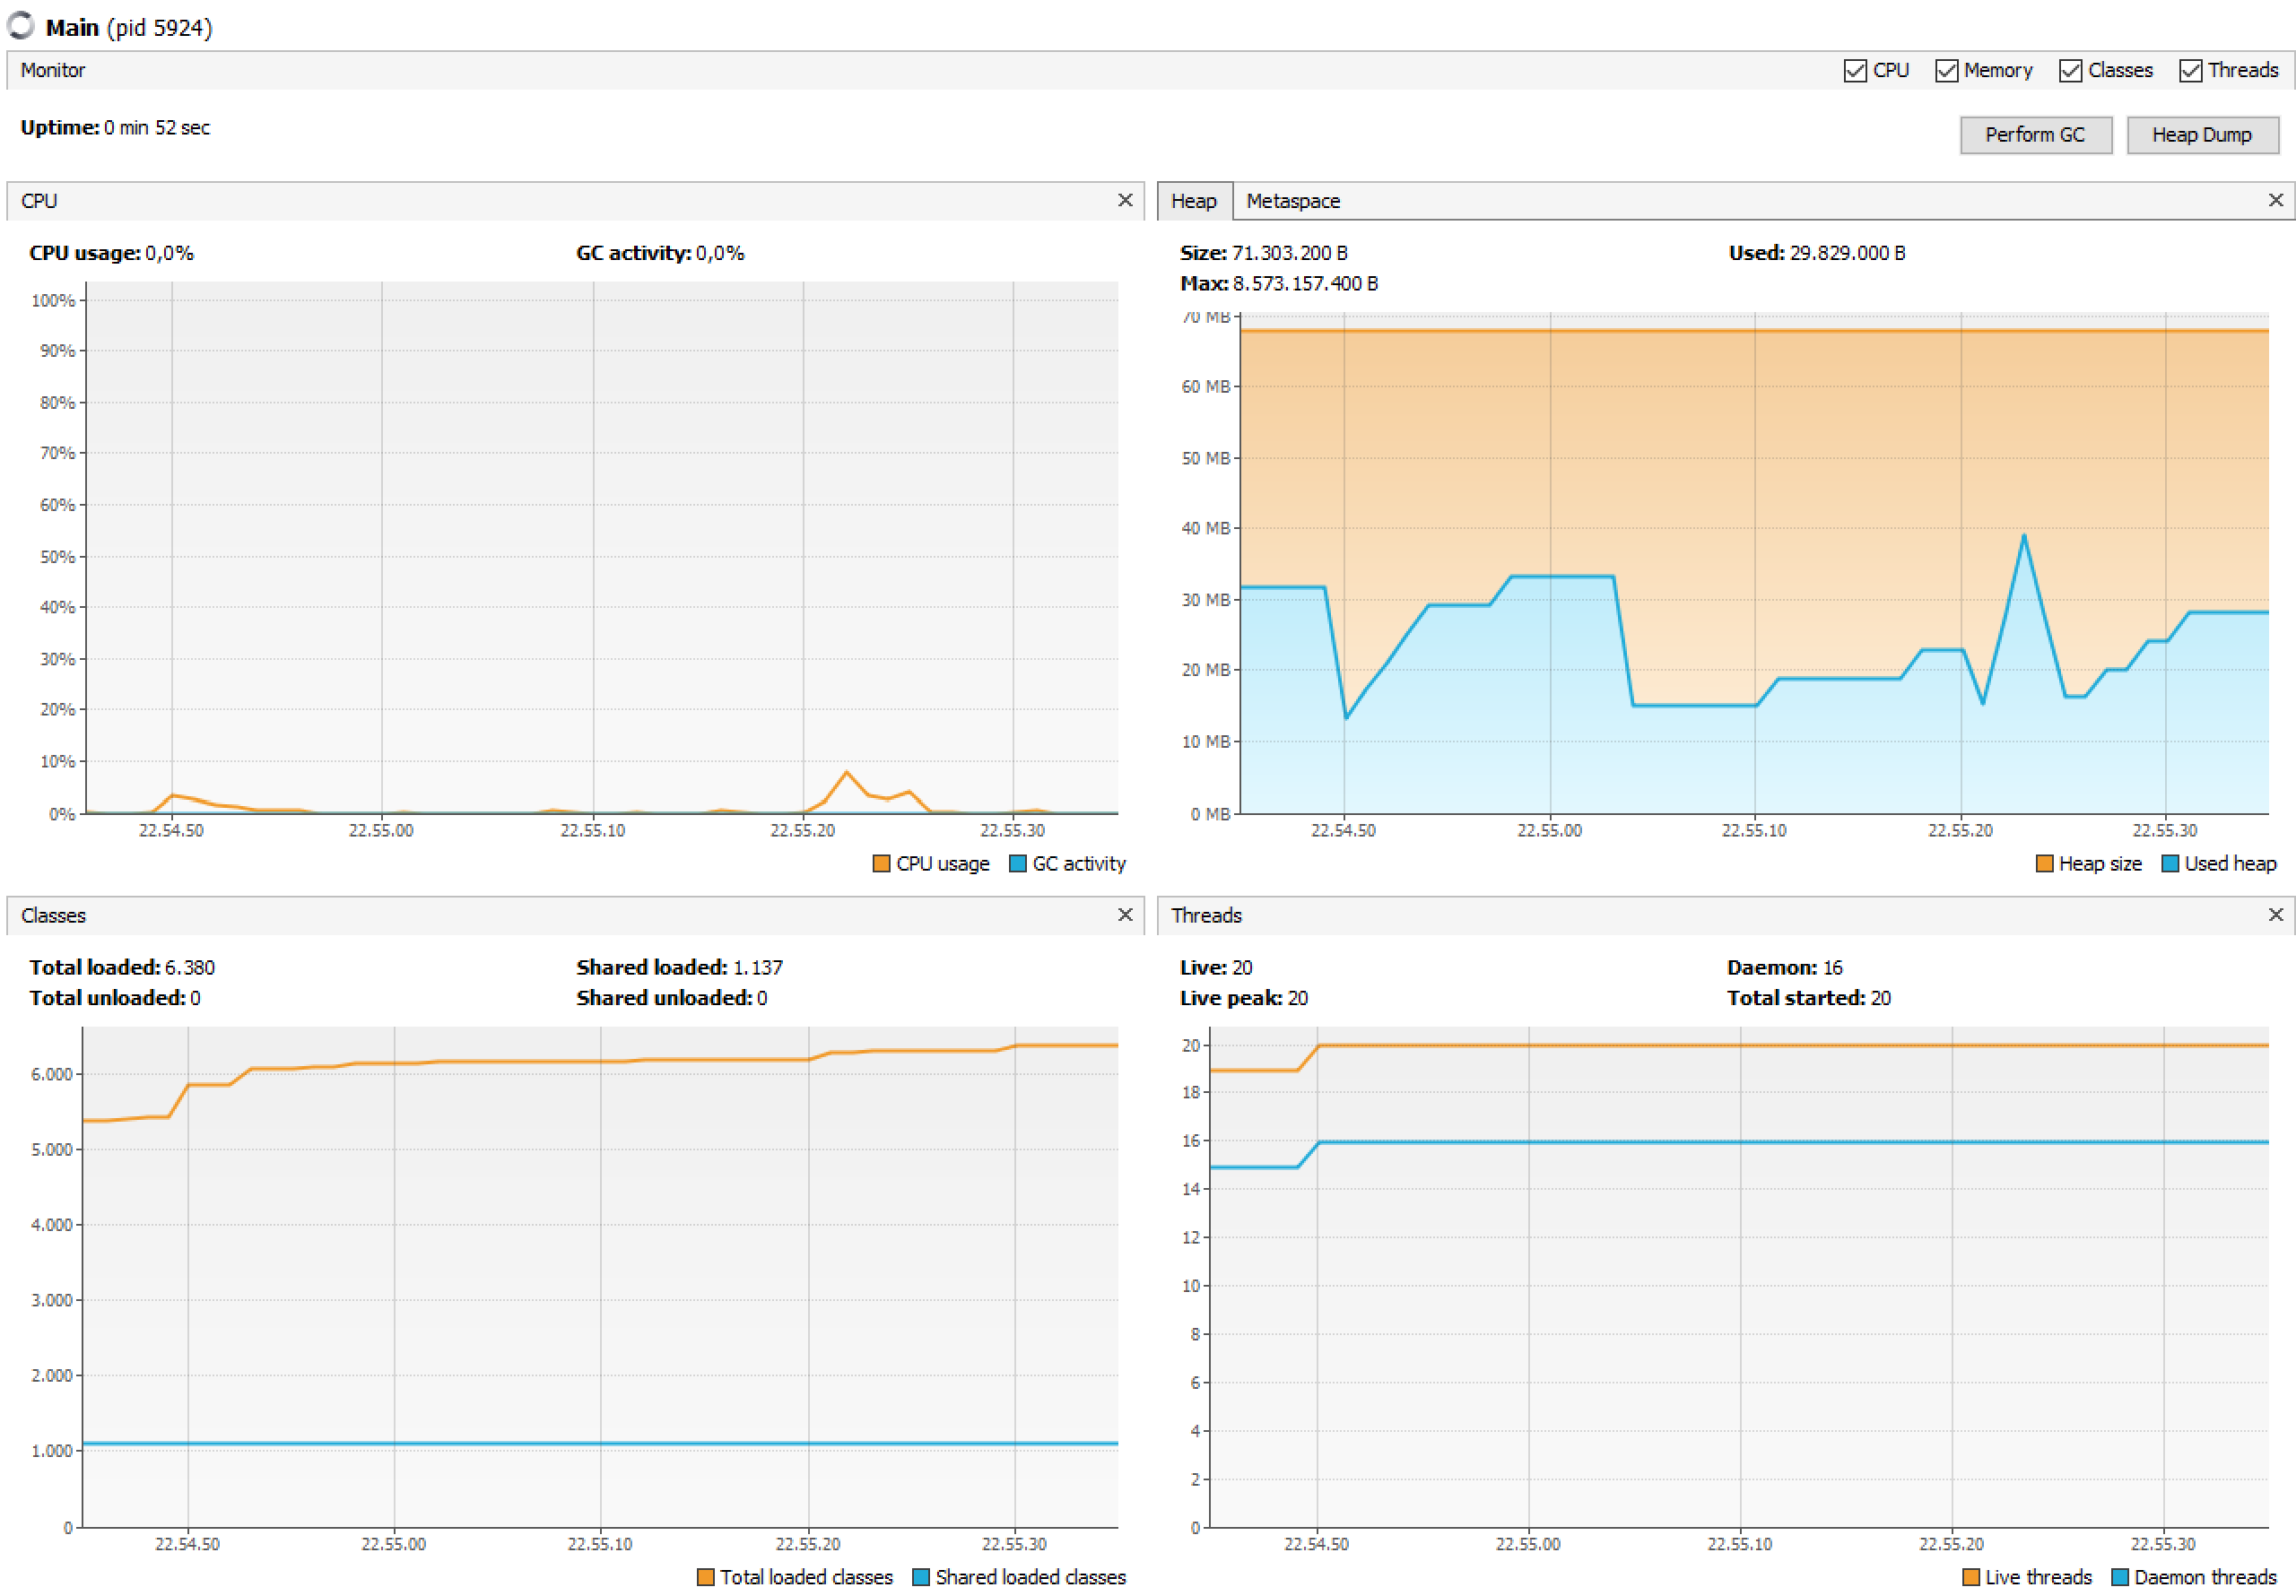
\includegraphics[width=\textwidth]{Images/VisualVM.png}
        \caption{Monitoraggio esecuzione di una partita}
        \label{fig:visualvm}
    \end{figure}